In this section we summarize the tests on fit behavior using data. 
First, we invetigate fit behaviors in the control regions. 
Second, the change in nuiscance parameters by nominal fit is examined.  

%%%%%%%%%%%%%%%%%%%%%%%%%%%%%%%%%%%%%%%%%%%
\subsection{Control region}
There are following control regions where we can do the tests.

\begin{itemize}
    \item{\textbf{Same-sign $e\M$/$\M e$ events} \\}  
        The sign requirement on the leptons is flipped. 
        This contral region is dominated by W+jets($e/\M$), \wgamma, \Wgstar, and WZ/ZZ.
    \item{\textbf{Same-sign \M\M~events} \\}  
        The sign requirement on the leptons is flipped. To get more statistics, 
        events in $|\mll - \mZ| < 15 \GeV$ are includeid. Instead of DYMVA, $minMET>35\GeV$
        is applied because requiring same sign reduces DY contribution (i.e. charge flip rate
        of muons is very small). This contral region is dominated by W+jets(\M), \Wgstar, and WZ/ZZ.
    \item{\textbf{Top-enriched sample} \\} 
        The top-veto requirement is flipped. This control region is dominated by top, WW, and Wjets.
%    \item{\textbf{WW-enriched} : }
%        $\mll > 70~\GeV$ is applied. This control region is dominated by WW, top, and Wjets.
%    \item Tri-lepton : ...  
\end{itemize}

The rest of selections are identical to the 2D analysis at $\mHi=125\GeV$.
In each test we perform a Maximum Likelihood fit with signal strength floated 
and check how normalizations of signal and background change.
Since signal contains only opposite sign di-lepton pairs, we use these events as signal 
in the test on same sign \M\M~events. The full 8 TeV data($\mathcal{L}=\intlumiEightTeV$) is used for the study.

Here is the summary of tests. Details( tables and plots) can be found in the 
appendix~\ref{sec:appendix_fitvalidation}. 
\begin{itemize}
    \item{\textbf{Same-sign $e\M$/$\M e$ events} (Table \ref{tab:fitval_norm_ss_0j}) \\ }  
        All processes are stable except for \Wgstar which is pulled down by about 40 \%.  
    \item{\textbf{Same-sign \M\M~events} (Table \ref{tab:fitval_norm_ssmm_0j}) \\ }  
        Signal contribution is close to 0 after fit. This means fit is able to 
        get the correct normalization when signal does not exist. All background 
        processes stay within the input uncertainties(i.e. 30 \% for  \Wgstar ).   
    \item{\textbf{Top-enriched sample} (Table \ref{tab:fitval_norm_top_0j}-\ref{tab:fitval_norm_top_1j}) \\ }  
        In 0jet bin there is a cross-feeding between qqWW and top. Other processes are stable. 
        In 1jet bin signal changed by -200\%, but the size of signal with respect to the total background 
        is only 1 \%. Therefore, change in the signal component is not significant. 
        Shift in backgrounds is not significant except for top. 
        Given that 94\% of the total background is from top, fit adjusts top to match data.  
%    \item{\textbf{WW-enriche}(Table \ref{tab:fitval_norm_ww_0j}-\ref{tab:fitval_norm_ww_1j}) : } 
%    \item Tri-lepton : ...  
\end{itemize} 

The conclusion is that fit does not show any anomalous behavior
when it is performed on the two control samples. Fit is able to assign 
proper normalizations of processes based on data.   

%%% SS 0jet
\begin{table}
\begin{center}
\begin{tabular}{c|cc|cc}
\hline
\hline
Process &    N(prefit) &   N(postfit) & Difference(yield) &  Difference(\%)  \\  
\hline
\hline
ZH &        1.7 &        0.2 &       -1.5 &      -89.4        \\
WH &        5.8 &        0.6 &       -5.2 &      -89.3        \\
qqH &        3.0 &        0.3 &       -2.7 &      -89.4        \\
ggH &      237.4 &       25.4 &     -212.0 &      -89.3        \\
\hline
qqWW &       14.1 &       20.5 &        6.5 &       46.1        \\
ggWW &        0.5 &        0.0 &        0.0 &        0.0        \\
\hline
VV &      104.7 &      107.3 &        2.6 &        2.5        \\
\hline
Top &        2.3 &        1.0 &       -1.3 &      -54.9        \\
\hline
Wjets($e$) &      136.8 &      122.5 &      -14.3 &      -10.4        \\
Wjets($\mu$) &      112.7 &      105.8 &       -6.9 &       -6.1        \\
\hline
W$\gamma$ &      100.5 &      109.0 &        8.5 &        8.5        \\
W$\gamma$* &      122.3 &       69.5 &      -52.8 &      -43.2        \\
\hline
Ztt &        0.1 &        0.0 &        0.0 &        0.0        \\
\hline
\hline
\end{tabular}
\caption{Pre- and post-fit normalizations in same sign $e\M$/$\M e$ events in 0jet bin. }
\label{tab:fitval_norm_ss_0j}
\end{center}
\end{table}

%%% SS mm 0jet
\begin{table}
\begin{center}
\begin{tabular}{c|cc|cc}
\hline
\hline
Process &    N(prefit) &   N(postfit) & Difference(yield) &  Difference(\%)  \\  
\hline
\hline
ZH &        0.9 &        0.0 &        0.0 &        0.0        \\
WH &        3.4 &        0.0 &       -3.4 &     -100.0        \\
qqH &        1.5 &        0.0 &       -1.5 &     -100.0        \\
ggH &      129.3 &        0.0 &     -129.2 &     -100.0        \\
\hline
qqWW &        0.1 &        0.0 &        0.0 &        0.0        \\
ggWW &        0.0 &        0.0 &        0.0 &        0.0        \\
\hline
VV &       54.1 &       58.1 &        4.0 &        7.4        \\
\hline
Top &        1.0 &        0.0 &        0.0 &        0.0        \\
\hline
Wjets($e$) &        0.0 &        0.0 &        0.0 &        0.0        \\
Wjets($\mu$) &       78.9 &       79.7 &        0.8 &        1.0        \\
\hline
W$\gamma$ &        0.0 &        0.0 &        0.0 &        0.0        \\
W$\gamma$* &       53.5 &       63.3 &        9.8 &       18.4        \\
\hline
Ztt &        0.0 &        0.0 &        0.0 &        0.0        \\
\hline
\hline
\end{tabular}
\caption{Pre- and post-fit normalizations in same sign \M\M~events in 0jet bin. }
\label{tab:fitval_norm_ssmm_0j}
\end{center}
\end{table}


%%% Top-enriched 0jet
\begin{table}
\begin{center}
\begin{tabular}{c|cc|cc}
\hline
\hline
Process     &    N(prefit) &   N(postfit) & Difference(raw) &  Difference(\%)  \\  
\hline
\hline
ZH &        0.2 &        0.0 &        0.0 &        0.0        \\
WH &        0.8 &        0.0 &        0.0 &        0.0        \\
qqH &        0.2 &        0.0 &        0.0 &        0.0        \\
ggH &        7.8 &        0.0 &       -7.8 &     -100.0        \\
\hline
qqWW &      137.2 &      197.8 &       60.6 &       44.2        \\
ggWW &        7.9 &        8.8 &        0.9 &       11.9        \\
\hline
VV &       18.8 &       17.1 &       -1.8 &       -9.3        \\
\hline
Top &      511.6 &      448.8 &      -62.8 &      -12.3        \\
\hline
Zjets &        0.0 &        0.0 &        0.0 &        0.0        \\
\hline
Wjets($e$) &       20.2 &       19.8 &       -0.4 &       -1.9        \\
Wjets($\mu$) &       35.5 &       42.5 &        7.0 &       19.7        \\
\hline
W$\gamma$ &        2.7 &        2.4 &       -0.4 &      -13.2        \\
W$\gamma$* &       41.5 &       44.1 &        2.7 &        6.5        \\
\hline
Ztt &        4.3 &        4.5 &        0.2 &        4.3        \\
       \hline
\hline
\end{tabular}
\caption{Pre- and post-fit normalizations in the top-enriched region in 0jet bin.}
\label{tab:fitval_norm_top_0j}
\end{center}
\end{table}

%%% Top-enriched 1jet
\begin{table}
\begin{center}
\begin{tabular}{c|cc|cc}
\hline
\hline
Process     &    N(prefit) &   N(postfit) & Difference(raw) &  Difference(\%)  \\  
\hline
\hline
ZH &        0.5 &        0.0 &        0.0 &        0.0        \\
WH &        1.1 &        3.5 &        2.4 &      220.5        \\
qqH &        1.2 &        4.0 &        2.7 &      220.3        \\
ggH &       10.7 &       32.9 &       22.2 &      208.1        \\
\hline
qqWW &      160.1 &      195.9 &       35.7 &       22.3        \\
ggWW &        6.1 &        6.2 &        0.0 &        0.6        \\
\hline
VV &       32.6 &       32.4 &       -0.2 &       -0.5        \\
\hline
Top &     5693.2 &     5388.5 &     -304.7 &       -5.4        \\
\hline
Wjets($e$) &       41.7 &       35.9 &       -5.8 &      -13.9        \\
Wjets($\mu$) &       75.2 &       81.0 &        5.8 &        7.7        \\
\hline
W$\gamma$ &        6.0 &        6.1 &        0.1 &        1.2        \\
W$\gamma$* &        9.2 &        9.6 &        0.3 &        3.8        \\
\hline
Ztt &       22.4 &       21.9 &       -0.5 &       -2.4        \\
\hline
\hline
\end{tabular}
\caption{Pre- and post-fit normalizations in the top-enriched region in 1jet bin.}
\label{tab:fitval_norm_top_1j}
\end{center}
\end{table}


%%%%%%%%%%%%%%%%%%%%%%%%%%%%%%%%%%%%%%%%%%%
\subsection{Impact of different WW shapes on the observed signal strength} 

In 2D analysis we rely on MC for WW shapes. We use Madgraph+Pythia6 as a central shape 
and MC@NLO+Herwig6 with/without QCD scale variations as alternate shapes to account for 
shape variation. Because it is hard to validate the WW shape against data, we perform 
nominal fit with different set of central and alternate shapes. If the changes in the 
signal strength($\mu$) is small by changing shapes, we are safe in accounting for shape uncertainties.
So, we define relative movement of signal strength with respect to the nominal one.   
The movement is defined as 
\begin{equation} 
|\Delta\mu| = \frac{|\mu_{nominal} - \mu_{variation}|}{|\mu_{nominal}|}  
\end{equation} 
where $\mu_{nominal}$ is from our choice for analysis and $\mu_{variation}$ is from 
different combination of samples. To remain blinded, we take absolute value of 
difference so that we are not aware of direction of changes. 
Table \ref{tab:fitval_mu} shows $\Delta\mu$ with two different choices of central 
and alternate shapes. Expected significance does not change. Maximum $\Delta\mu$ is 12\%.
Thus, we conclude that signal strength is not sensitive to the choice of WW MC.

%%% 
\begin{table}[ht!]
\begin{center}
\begin{tabular}{c|c|c|c}
\hline \hline
Central shape               & Madgraph          & Powheg            & MC\@NLO           \\  
\hline 
Different generator         & MC\@NLO           & MC\@NLO           & Madgraph          \\  
\hline
Scale variation             & MC\@NLO up/down   & MC\@NLO up/down   & MC\@NLO up/down   \\  
\hline \hline
Expected significance       & 3.5               & 3.5               & 3.6               \\  
$\Delta\mu$                 & 0                 & 3\%               & 12\%               \\  
\hline \hline
\end{tabular}
\caption{Shift in signal strength by different choice of central and alternate shapes.}
\label{tab:fitval_mu}
\end{center}
\end{table}


%%%%%%%%%%%%%%%%%%%%%%%%%%%%%%%%%%%%%%%%%%%
\subsection{Validation of $qq\rightarrow\WW$ fit model}  

In 2D analysis we rely on simulation for background shapes. 
The most sensitive channel, 0jet DF, is dominated by $qq\rightarrow\WW$ process. 
Therefore, it is important to confirm that our fit model (shape and normalization) 
correctly describes data. In this section, we describe a study on this subject using two 
control regions dominated by $qq\rightarrow\WW$ process.
The basic idea is that if the fit model is not correct then the prediction using 
one region may not be compatible with that using another region. To test this, 
we use post-fit result in one control region and predict the shape and normalization 
in another region. Following is the procedure and the result of this test. 

We first select two control regions with similar statistics. It's important that 
both regions contain similar data events so that both regions have similar statisitical 
power to constrain backgrounds. 
%
\begin{figure}[!hbtp]
\centering
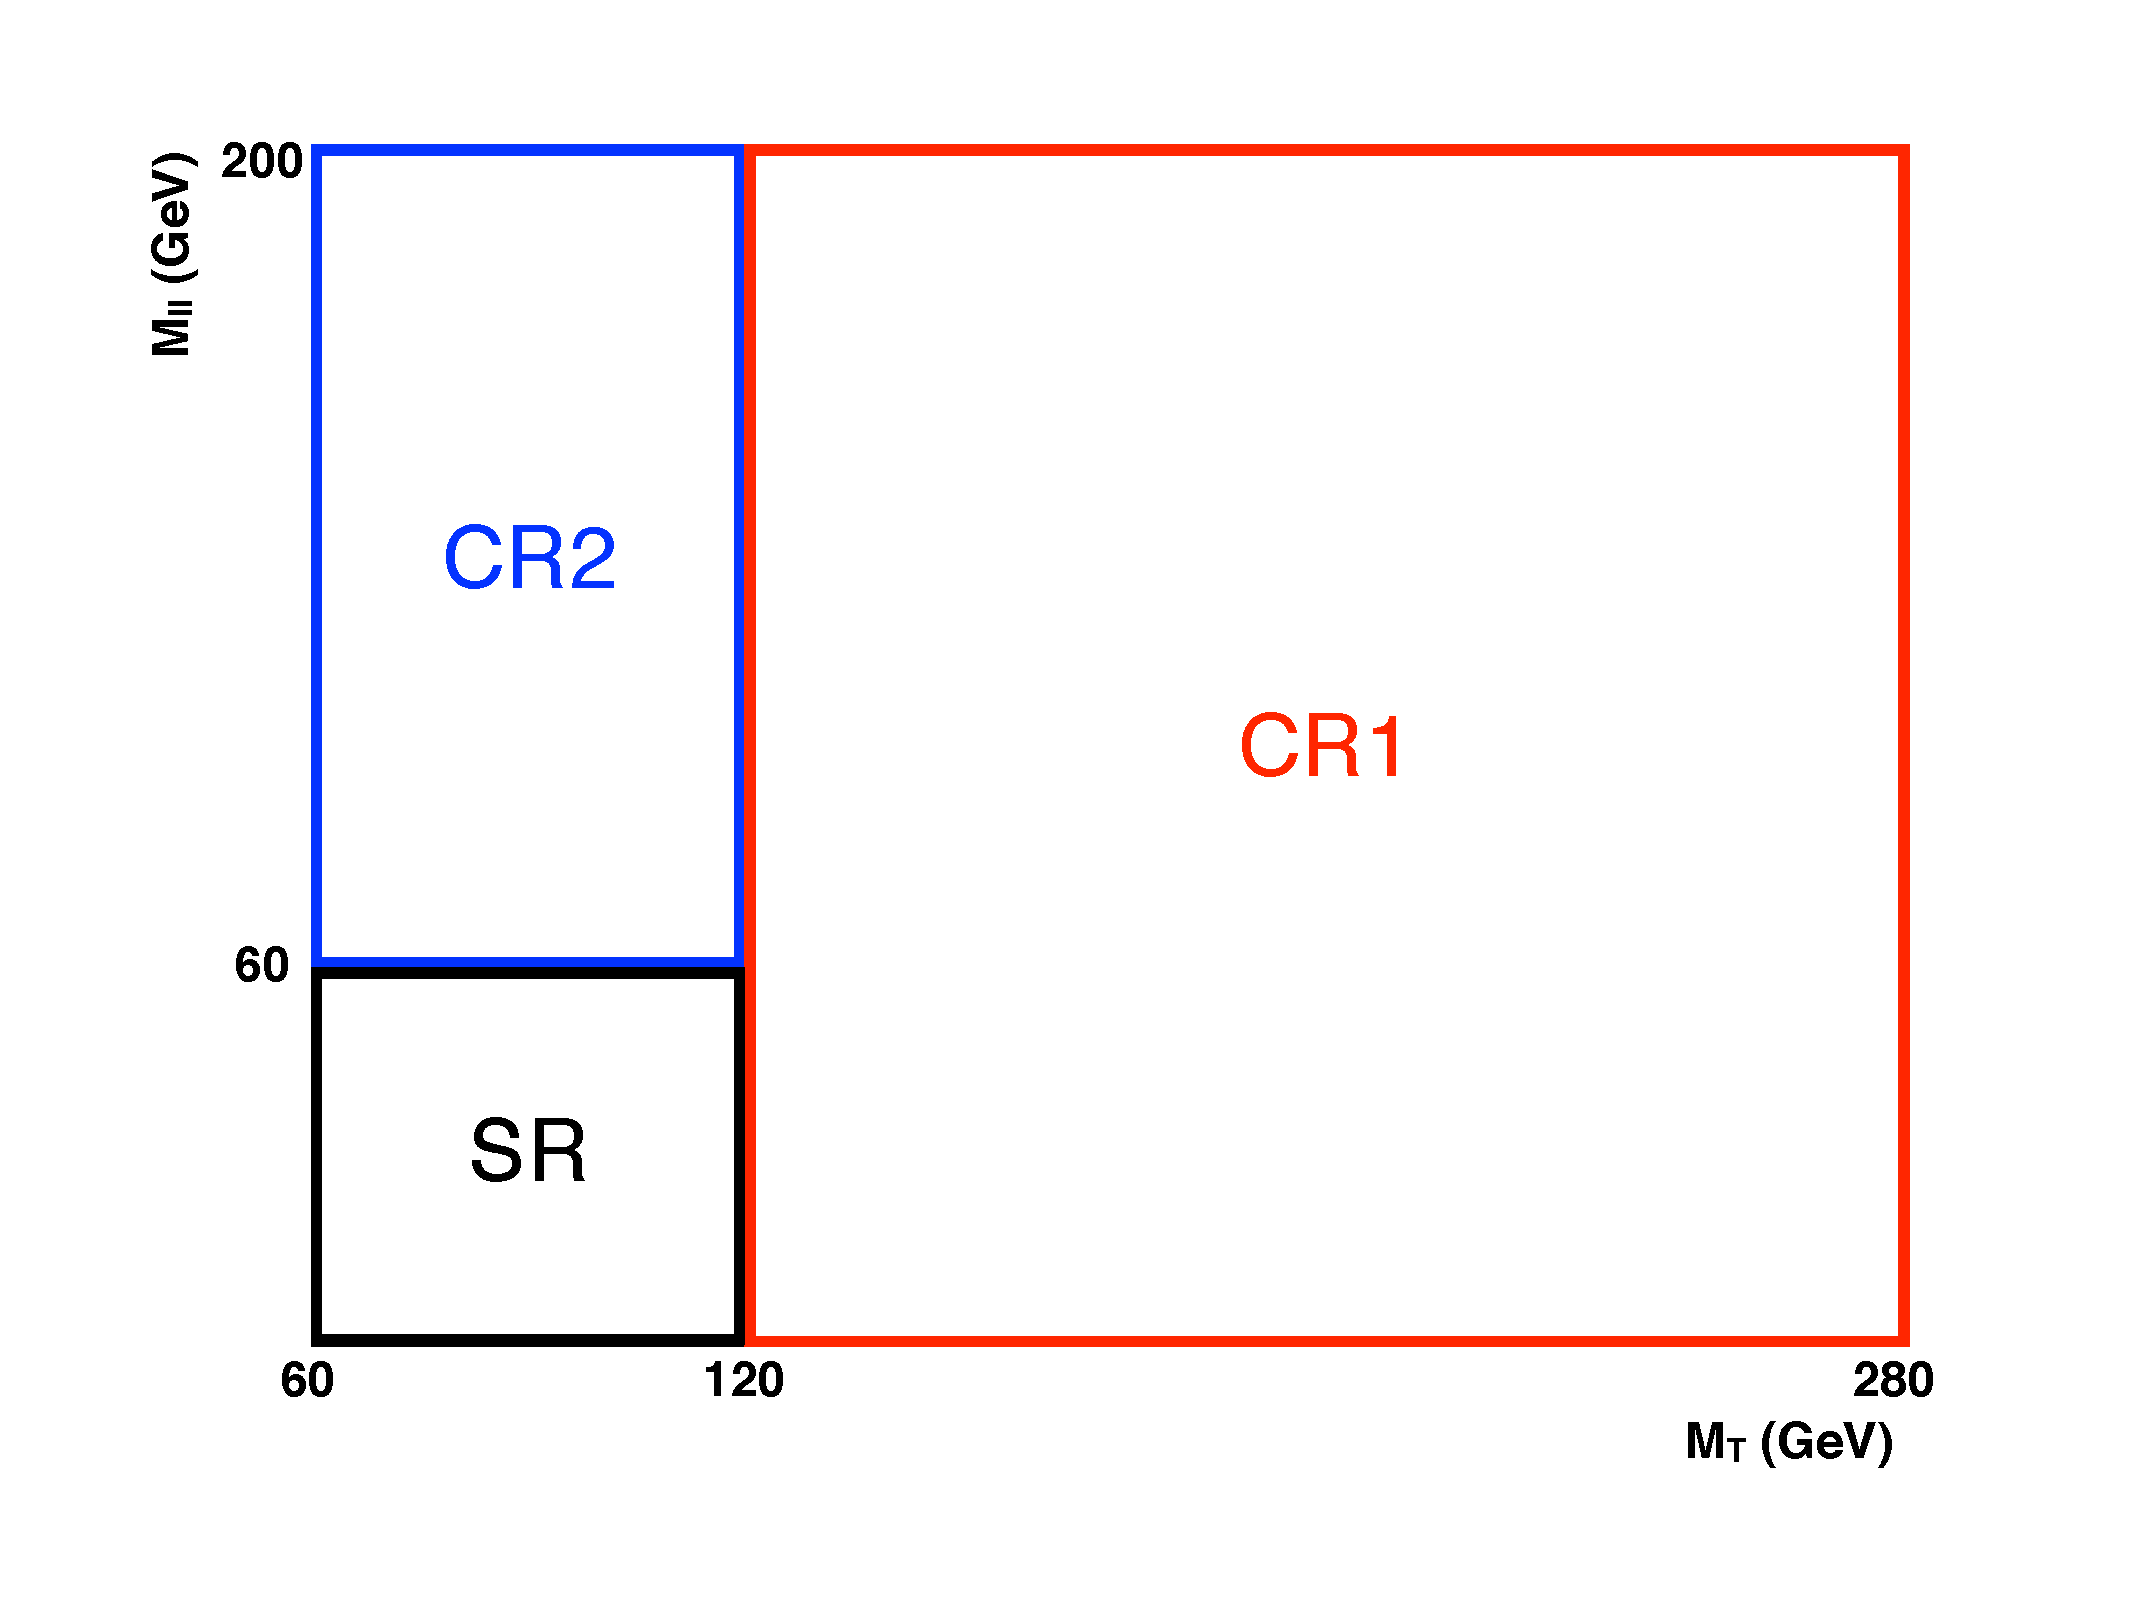
\includegraphics[width=.6\textwidth]{figures/WWctl_scheme.pdf}
\caption{Definition of signal region(SR), and two control regions(CR1 and CR2). 
SR is defined by $60<\mt<120~\GeV$ and $12<\mll<60~\GeV$. 
CR1 is defined by $120<\mt<280~\GeV$ and $12<\mll<200~\GeV$. 
CR2 is defined by $60<\mt<120~\GeV$ and $60<\mll<200~\GeV$. }
\label{fig:WWctlregions}
\end{figure}
Figure \ref{fig:WWctlregions} shows signal region(SR) which is drawn in black 
and two control regions, CR1 and CR2, which are drawn in red and in blue, respectively. 
SR is defined by $60<\mt<120~\GeV$ and $12<\mll<60~\GeV$. 
CR1 is defined by $120<\mt<280~\GeV$ and $12<\mll<200~\GeV$. 
CR2 is defined by $60<\mt<120~\GeV$ and $60<\mll<200~\GeV$. 
%
\begin{table}
\begin{center}
\begin{tabular}{c|cccccccccc|c}
\hline
Region & Signal & qqWW & ggWW & VV & Top & Wjets(e) & Wjets($\mu$) & W$\gamma$ & W$\gamma$* & Ztt & Data \\
\hline
CR1 & 27.0  &  1321.0 & 113.2 &  46.2  &  289.6 &  54.9  &  22.4 &   6.0& 19.3 &   2.8 &1892\\
CR2 & 13.5  & 1672.7 & 54.5   & 51.5  &  146.1 &  108.1 &  128.2 &  19.3 &   21.4  &  19.9 &   2155 \\
Full range & 238.4 &  3969.6 & 210.6 &  132.6 &  498.7 &  282.8 &  331.8 &  115.6  & 167.8 &  46.0 &   5729 \\
\hline
\end{tabular}
\end{center}
\caption{Definition of signal region(SR), and two control regions(CR1 and CR2).} 
\label{tab:WWctlregions_composition}
\end{table}
The composition of signal and backgrounds in the two control regions is summarized 
in Table \ref{tab:WWctlregions_composition}. Both regions are dominated by $qq\rightarrow\WW$
with purity of around 70(75)\% in CR1(2). Signal contamination is negligible (less than 1.5\%). 

Because this test is only on $qq\rightarrow\WW$, other processes have to be fixed in the fit.
We generate new cards with all processes fixed to post-fit normailzataion and shape except 
for $qq\rightarrow\WW$ process. The post-fit normalization and shapes are from a nominal fit. 
Hereafter, this card will be called ``full range" card. In the full range card, all nuisances for 
$qq\rightarrow\WW$ are included, but all nuisances for other processes are dropped because they are 
already post-fit results. 
%
\begin{figure}[!hbtp]
\centering
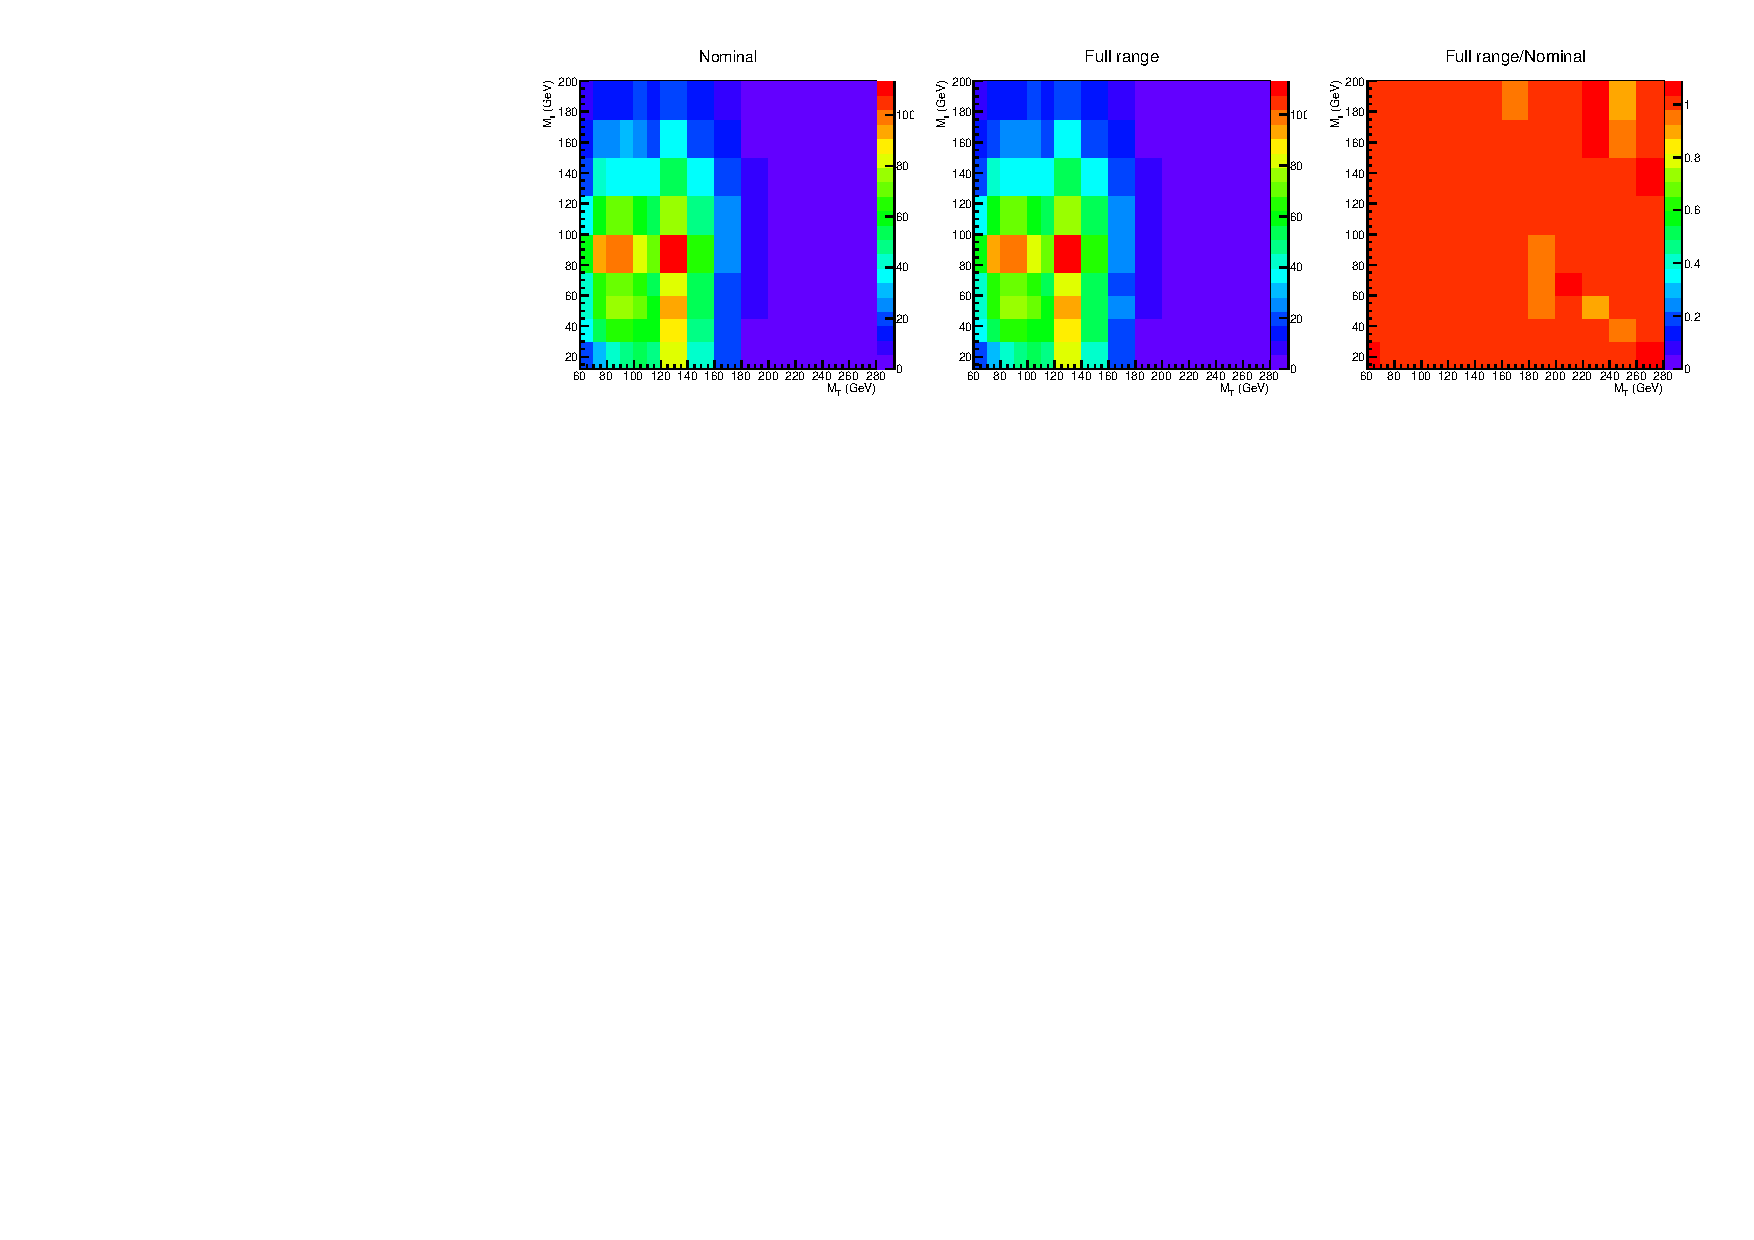
\includegraphics[width=1.0\textwidth]{figures/2Dshape_sanity.pdf} \\
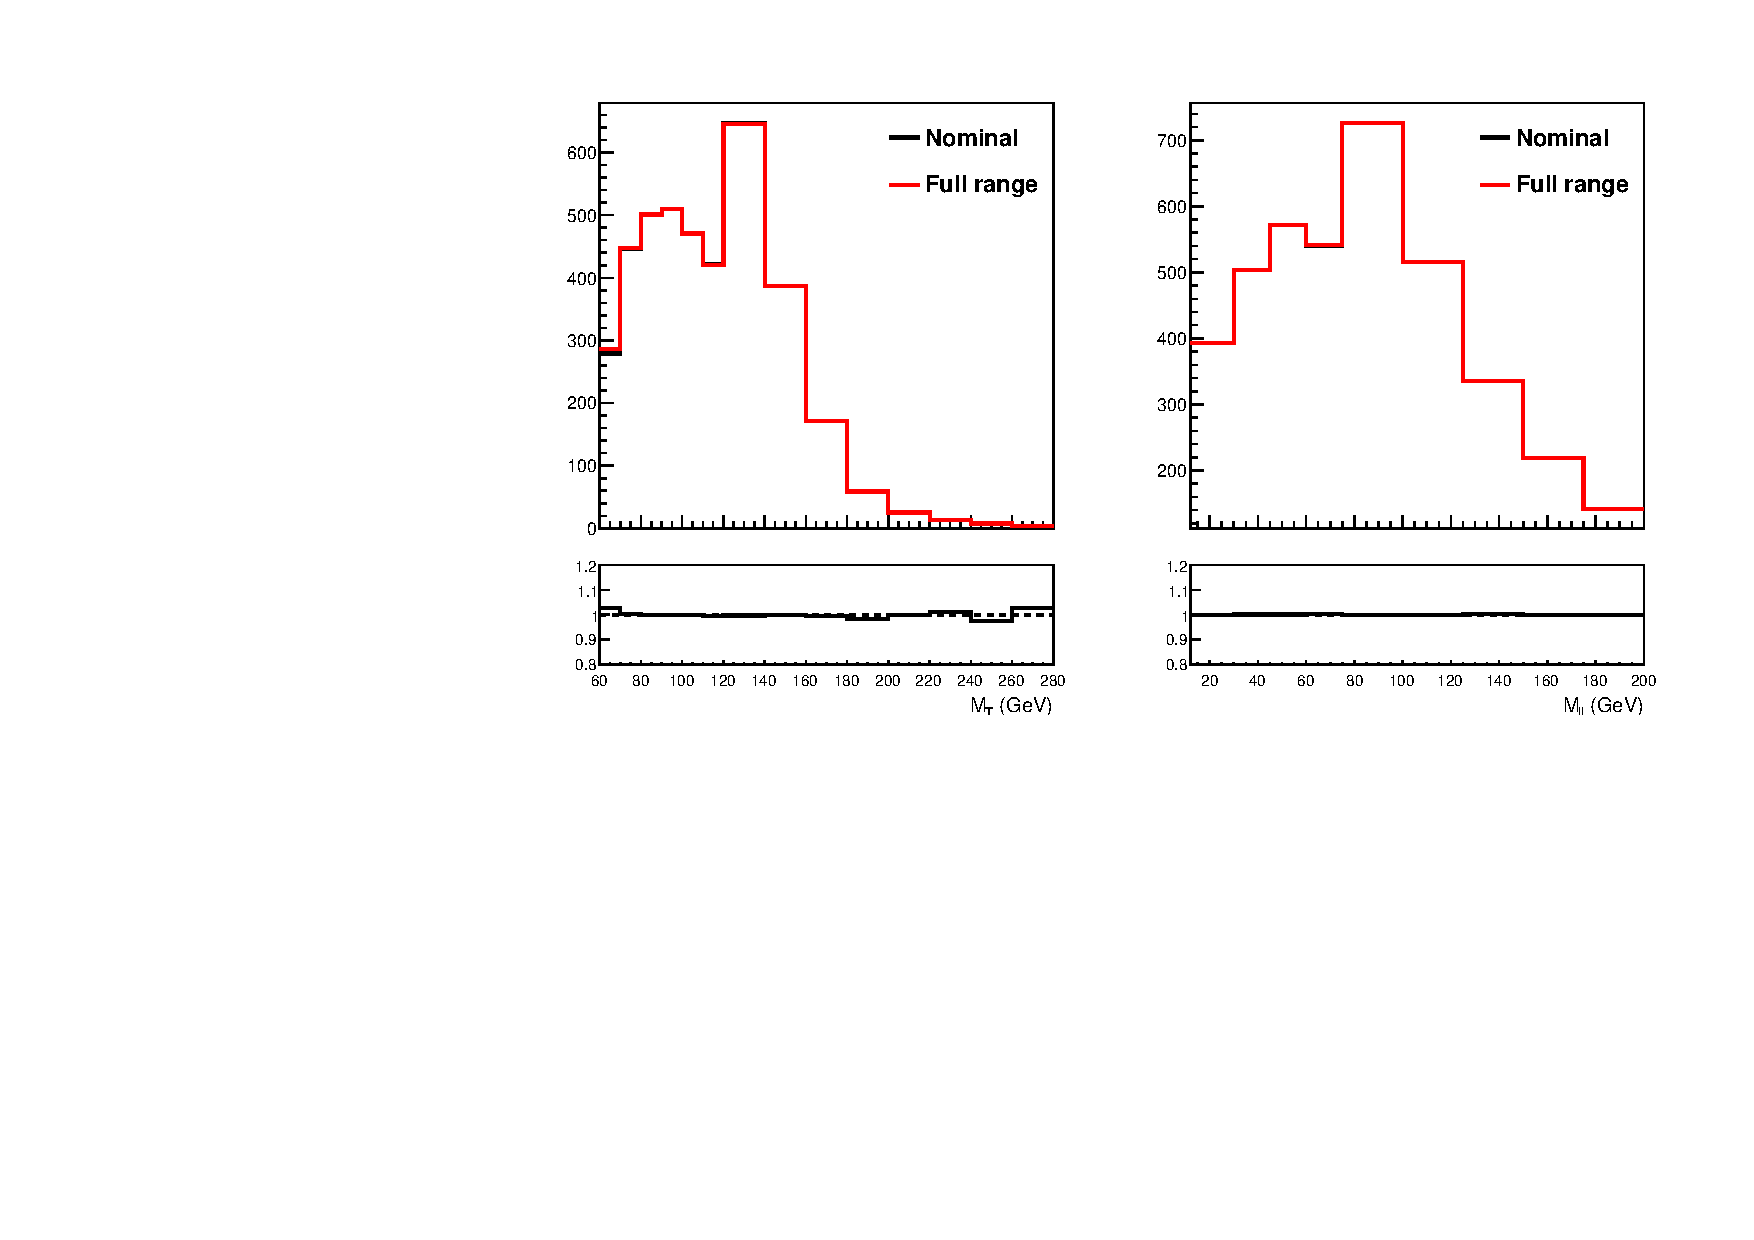
\includegraphics[width=.8\textwidth]{figures/1Dshape_sanity.pdf} 
\caption{Comparison of post-fit shapes of qqWW from nominal and full range fits. 
Top plots show individual 2D shapes and ratio(Full range/Nominal). 
Bottom plots show \mt~and \mll~projections.}
\label{fig:sanity_fullrange}
\end{figure}
%
\begin{table}
\begin{center}
\begin{tabular}{c|cccc}
\hline
Fit         & VH    & qqH   & ggH   & qqWW          \\
\hline
Nominal     & 4.8   & 1.9   & 144.3 &  3945.4       \\
Full range  & 4.8   & 1.9   & 143.6 &  3947.0       \\
\hline
\end{tabular}
\end{center}
\caption{Comparison of nomalization from nominal and full range fits.} 
\label{tab:sanity_fullrange}
\end{table}
As a sanity check we compare the post-fit shape and normalization 
using full range card with those using the nominal card in Figure \ref{fig:sanity_fullrange} and 
Table \ref{tab:sanity_fullrange}. Both shapes and normalizations using full range card 
are consistent with the nominal fit results. 

Since the full range card has been validated, we perform two fits using only one control region.
The fit using CR1(2) will be denoted as CR1(2) fit hereafter. In a fit using one control region, 
the other region is removed in the card and normalization is fixed accordingly. 
\begin{figure}[!hbtp]
\centering
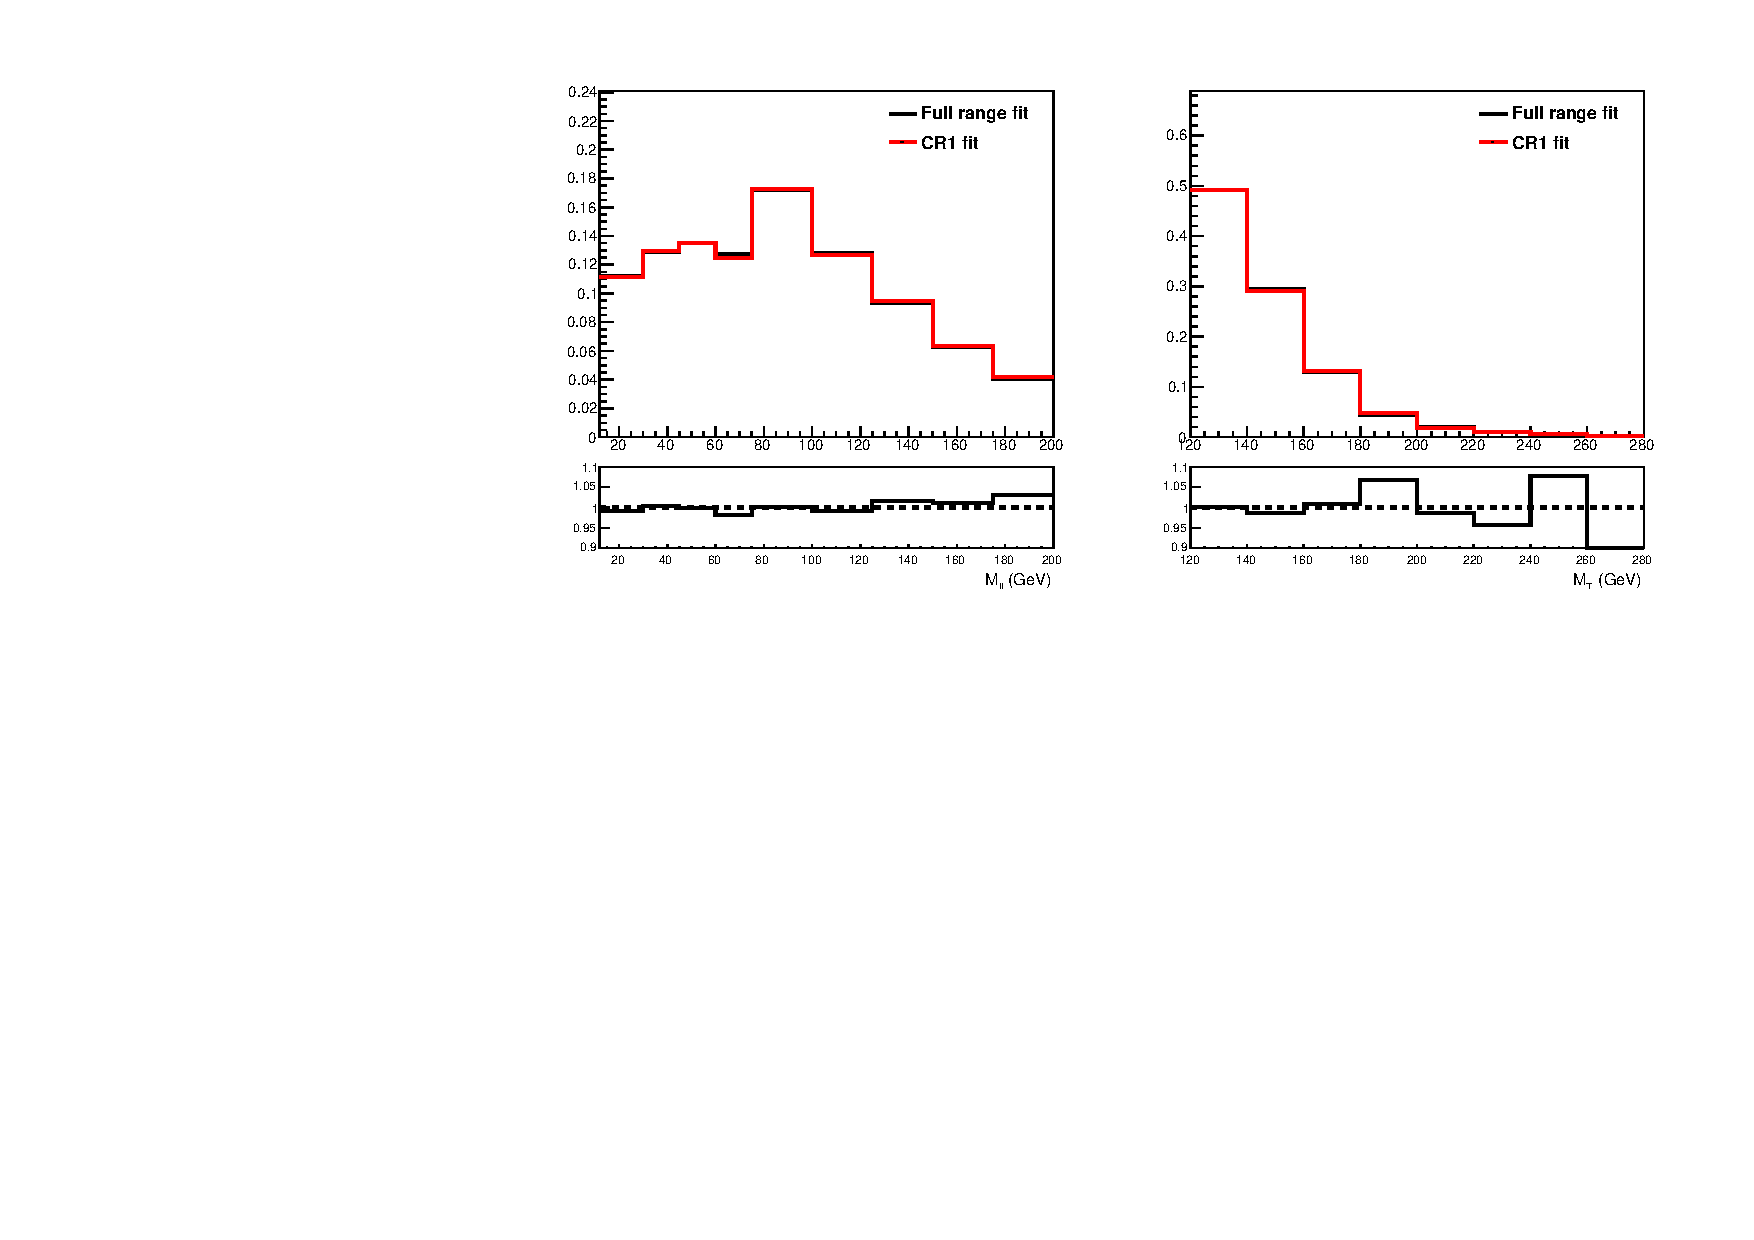
\includegraphics[width=.8\textwidth]{figures/1Dshape_CR1_plotCR1.pdf} \\
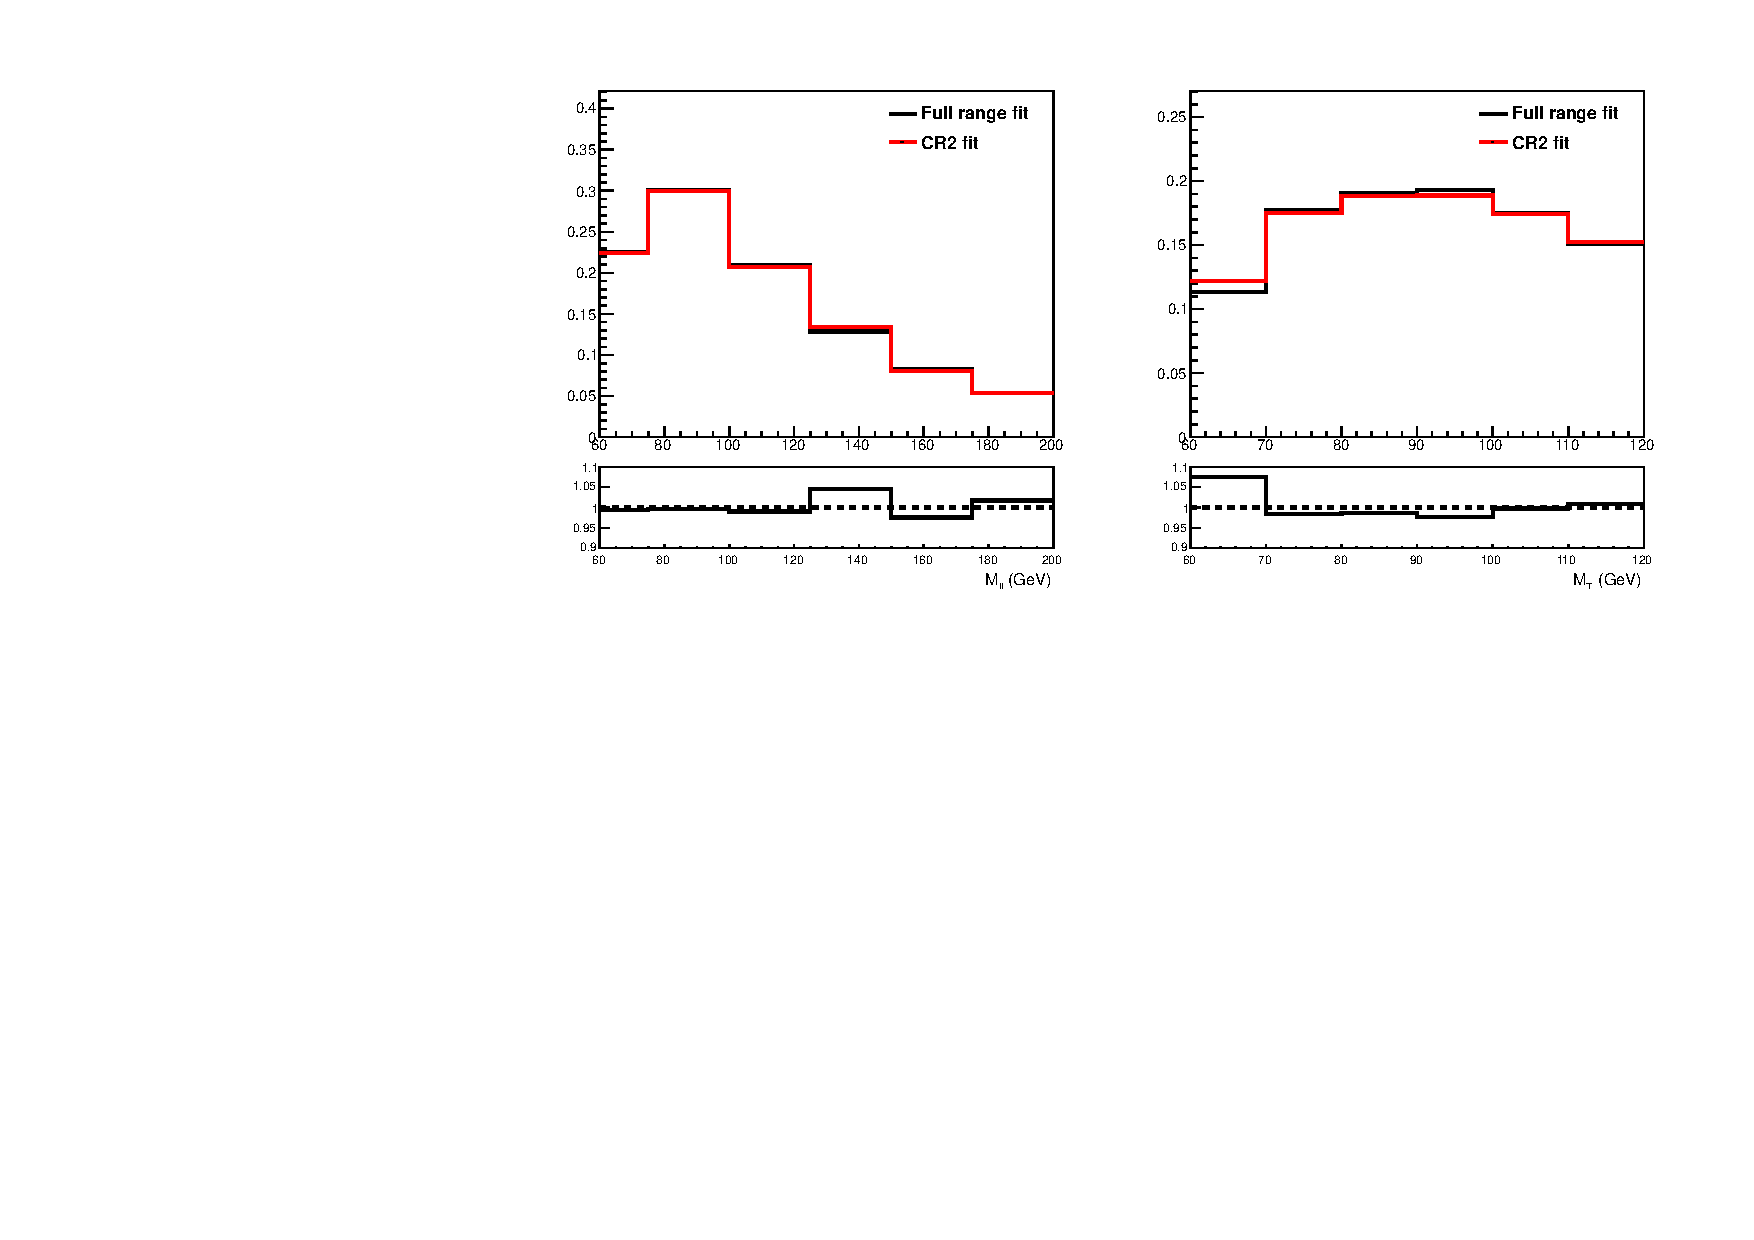
\includegraphics[width=.8\textwidth]{figures/1Dshape_CR2_plotCR2.pdf} 
\caption{Comparison of post-fit shapes from the CR1(2) and full range fits in 
red and black, respectively. Top plots are for CR1 fit and bottom plots are 
for CR2 fit. Plots are normalized to unit area.}
\label{fig:sanity_fullrangeandcr}
\end{figure}
Figure \ref{fig:sanity_fullrangeandcr} shows post-fit \mt~and \mll~distributions  
from CR1(2) and full range fits. Plots are normalized to unit area to compare only shapes. 
In both fits in the two control regions, shapes are consistent with those of the full range fit.
Using this result, we can draw one control region using the post-fit normalization  
from the other control region. For example, we can draw CR1 by renormalizing
post-fit qqWW distribution from full range fit to the post-fit normalization of the CR2 fit
in CR2. Same procedure can be followed to draw CR2.

\begin{figure}[!hbtp]
\centering
\subfigure[\mll~in CR1]{
\centering
\label{subfig:cr1_mll}
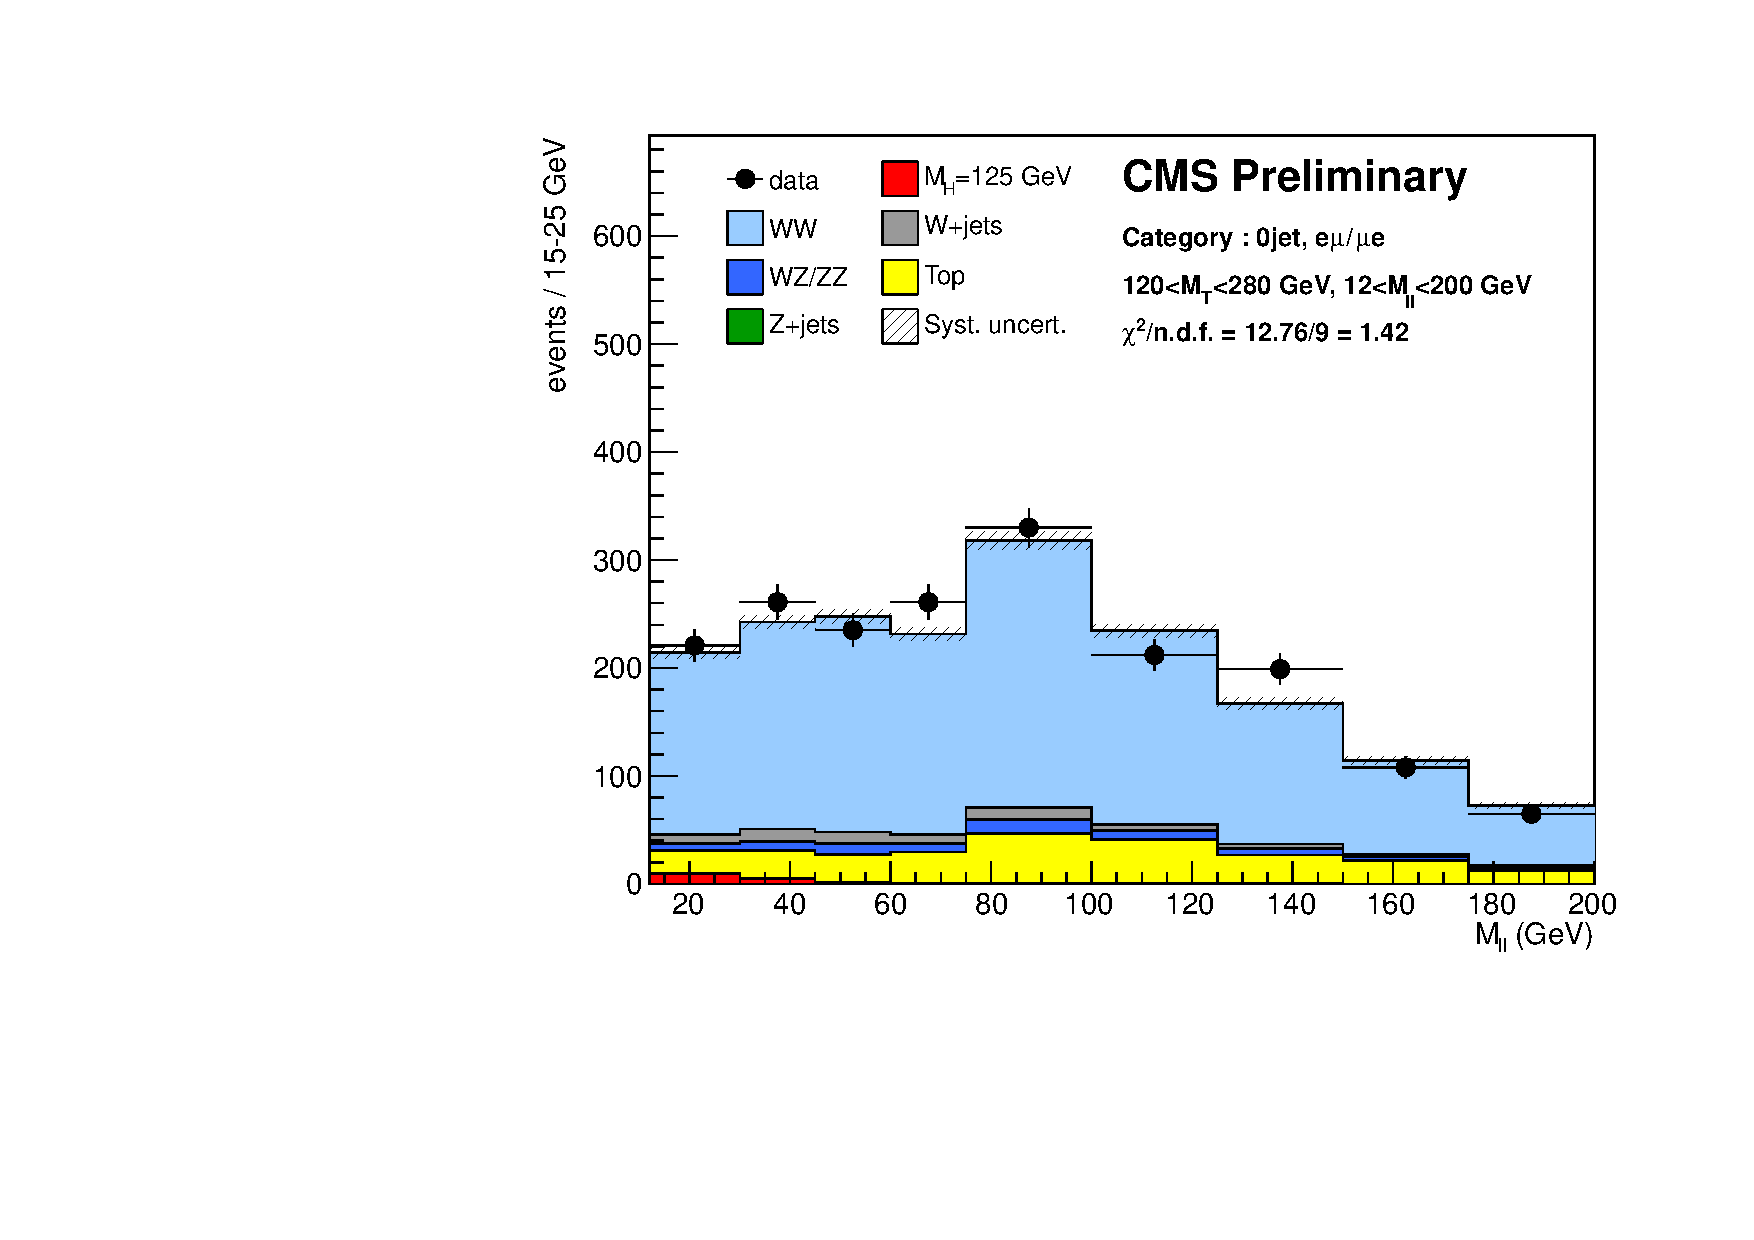
\includegraphics[width=.45\textwidth]{figures/mll_CR1_weightedqqww.pdf}
}
\subfigure[\mt~in CR1]{
\centering
\label{subfig:cr1_mT}
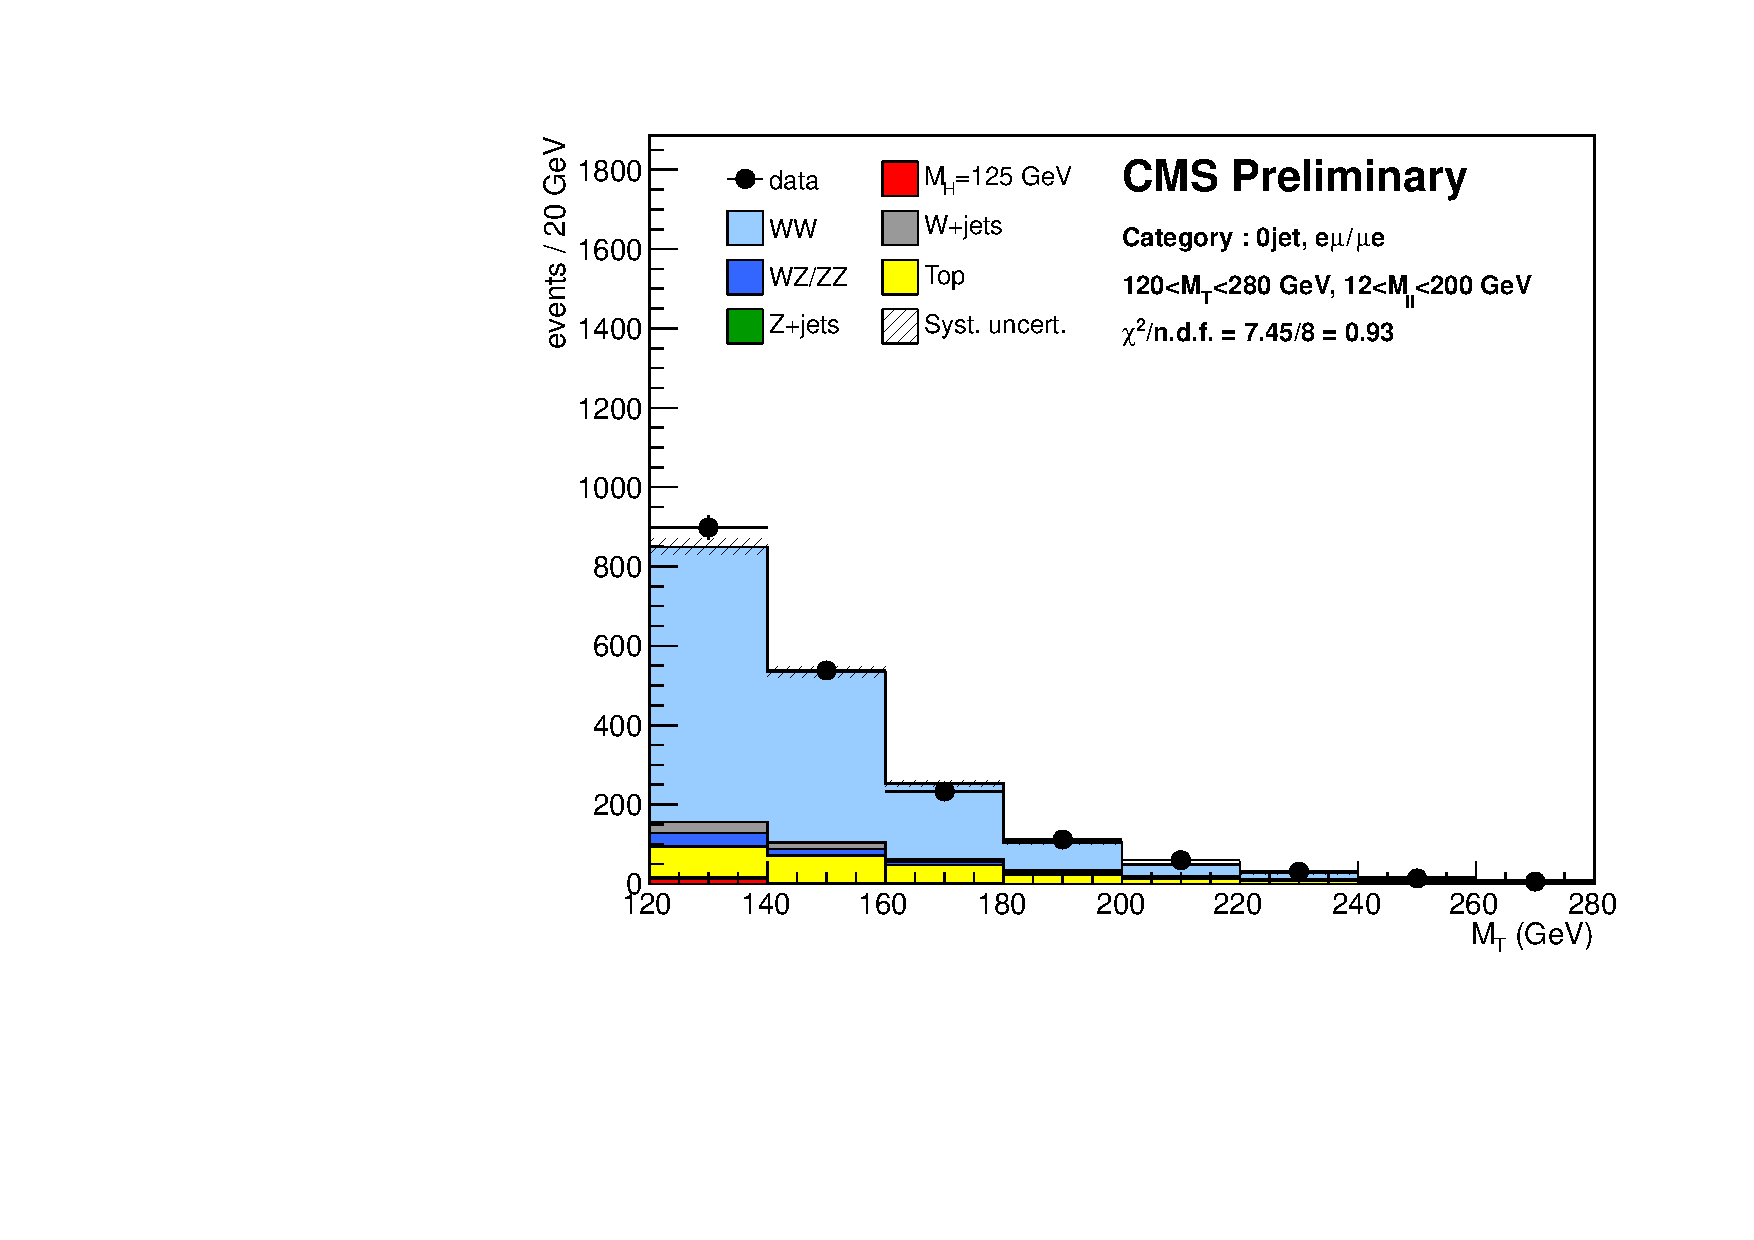
\includegraphics[width=.45\textwidth]{figures/mT_CR1_weightedqqww.pdf}
}\\
\subfigure[\mll~in CR2]{
\centering
\label{subfig:cr2_mll}
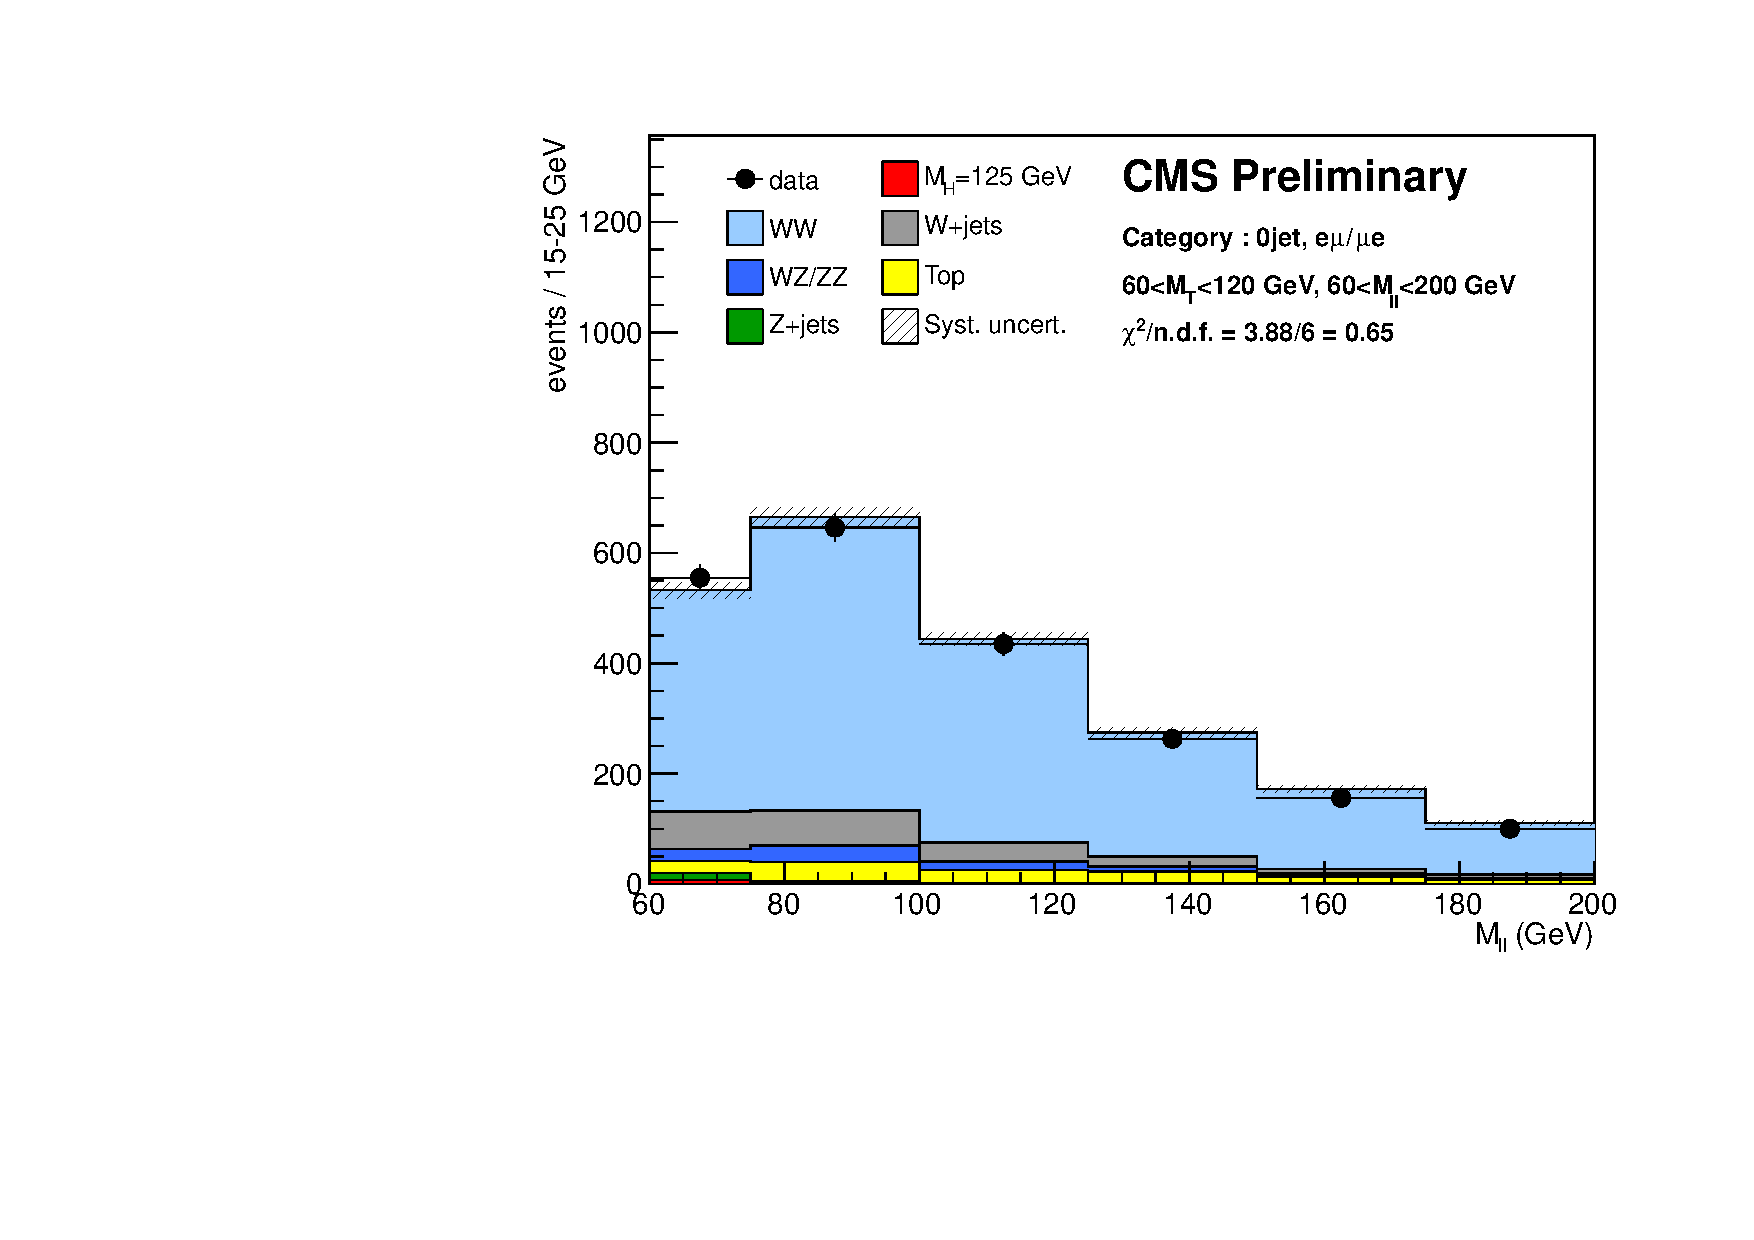
\includegraphics[width=.45\textwidth]{figures/mll_CR2_weightedqqww.pdf}
}
\subfigure[\mt~in CR2]{
\centering
\label{subfig:cr2_mT}
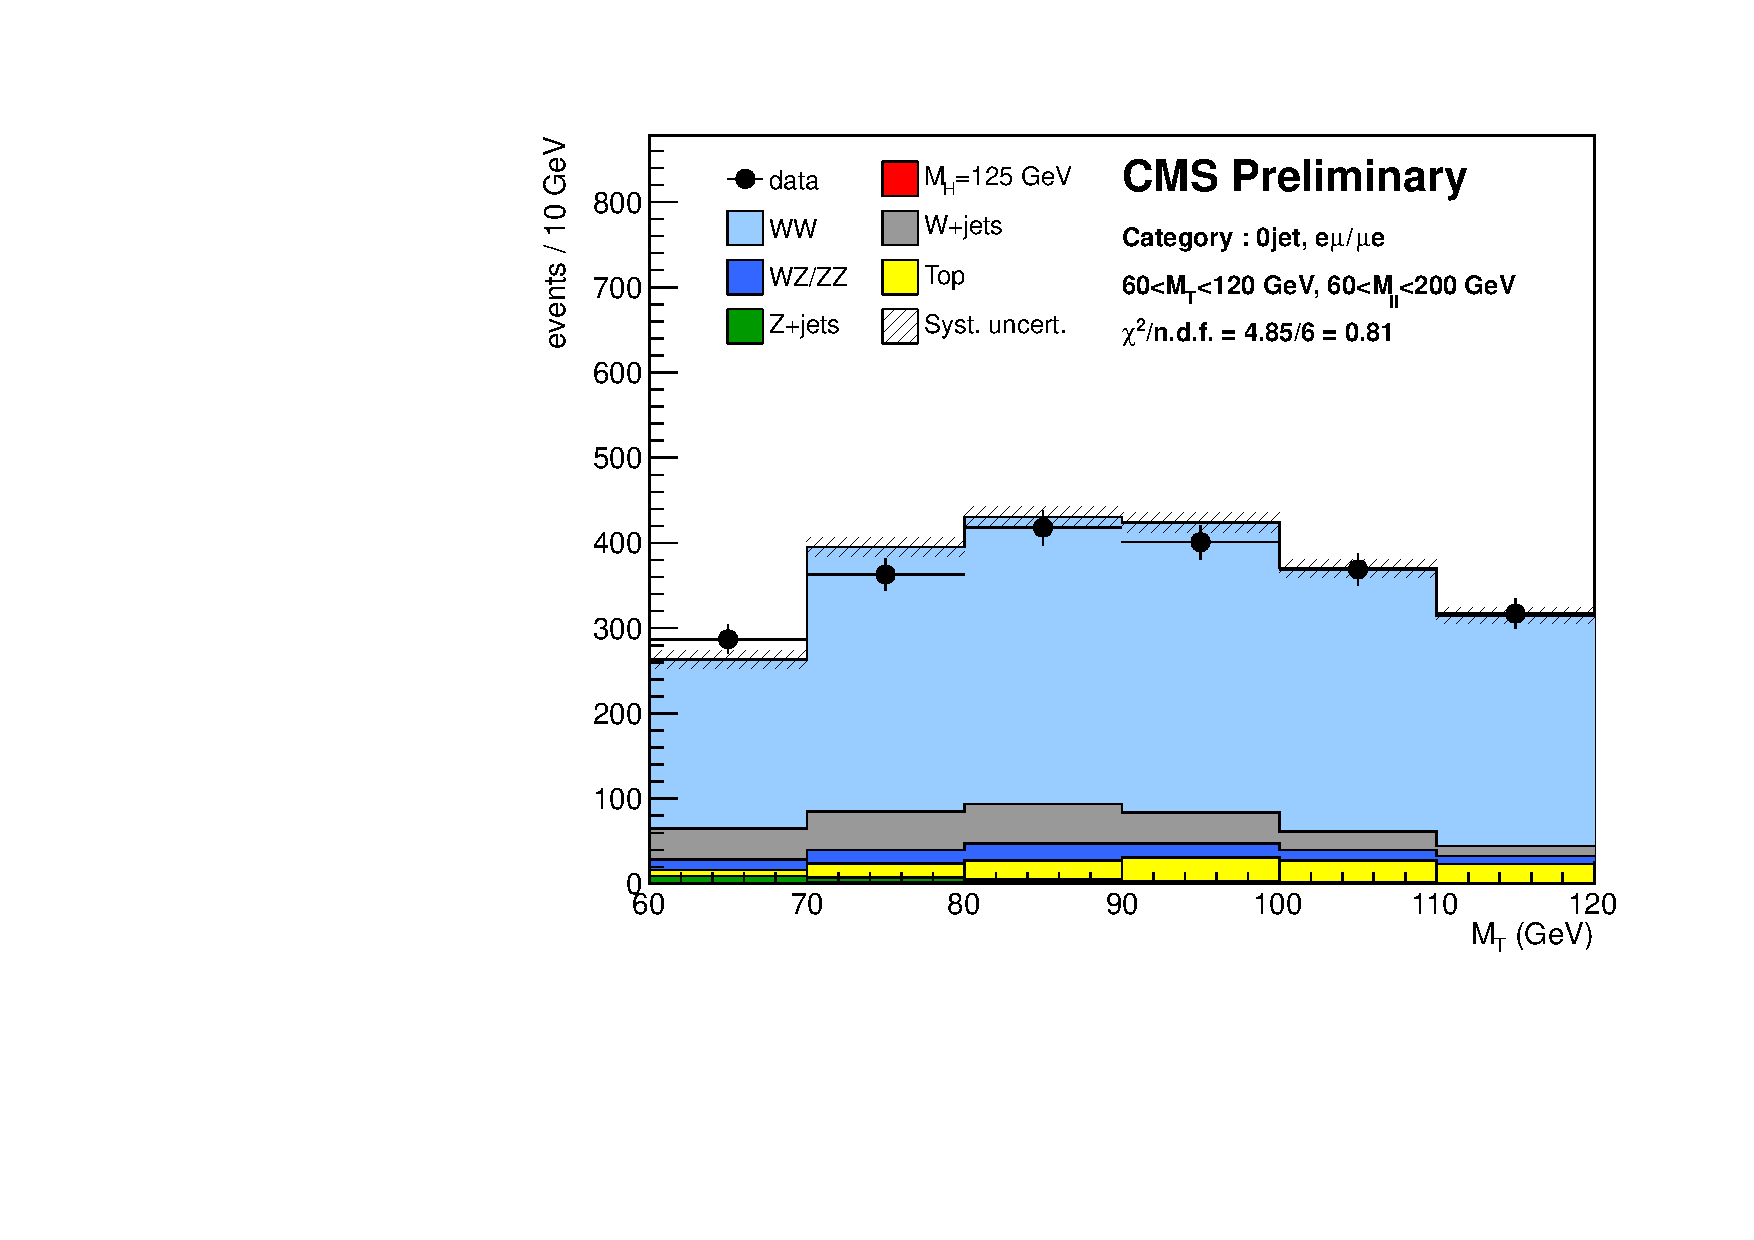
\includegraphics[width=.45\textwidth]{figures/mT_CR2_weightedqqww.pdf}
}\\
\caption{\mt~and \mll~plots in CR1(top) and CR2(bottom) using normalization
of the other control region.}
\label{fig:wwctl_final}
\end{figure}

Figure \ref{fig:wwctl_final} shows \mt~and \mll~distributions in CR1 and CR2 using 
normalizations from the other control regions. The uncertainty band is from pseudo-data 
sets generated using the full range card. Variances in each bin of qqWW and all other 
backgrounds are taken from full range and the nominal fits, repectively, and added in quadrature. 
The agreement between data and prediction is measured by $\chi^2/n.d.f.$ which is 
shown on each plot. All distributions show good agreement with data.
This indicates that our qqWW fit model is not biased.
%
\begin{table}
\begin{center}
\begin{tabular}{c|ccc}
\hline
                    & full range fit    & CR1 fit   & CR2 fit   \\
\hline
Best-fit $\mu$      & 0.63              & 0.63      & 0.62      \\
\hline
\end{tabular}
\end{center}
\caption{Comparison of the best-fit $\mu$ values from nominal, full range, CR1 and CR2 fits.} 
\label{tab:bestfitmu_compare}
\end{table}
Table \ref{tab:bestfitmu_compare} shows the best-fit $\mu$ values from full range, 
CR1 and CR2 fits. Using different control regions results in consistent best-fit $\mu$ values. 
This is an another evidence that our fit model is correct. 

Therefore, we conclude that our fit model for qqWW process correctly fits data.  
